To evaluate our state estimation, we compare approaches and parameter sensitivities with respect to the accuracy, robustness and flexibility requirements defined in section \ref{sec:design-requirements}. We use real measurement data from previous testing sessions with the \gls{dv} vehicle, recorded directly from the \gls{can} bus, making the evaluation realistic. We embed the state estimation into a simulation environment, which loads the measurement data and feeds them into the state estimation model. It also generates signals for the time since the arrival of the last measurement based on the signal frequency, since these are not included in the measurement data. Additionally, sensor failures can be injected.


\section{Results}
A fundamental problem with evaluation of state estimations is the lack of ground truth data, which only a vehicle simulation could provide. Since we do not have access to one, we resort to a visual inspection based on physical knowledge. For the \gls{ekf}, we additionally analyze the residuals, since non-zero mean residuals indicate a model--reality mismatch~\cite[p.~158]{AlexanderWischnewski.2019}. We will now show simulation results from all three stages of the state estimation.


\subsection{IMU Fusion}
The \gls{imu} fusion is the only part of the preprocessing stage we will evaluate, since everything else is straightforward physical transformations. Figure \ref{fig:imu-fusion-real} shows the input measurements from two \glspl{imu} mounted about \SI{80}{\centi\meter} in front and behind \gls{cog} (see section \ref{sec:design-sensor-setup}) as well as the result of their mean-based fusion. The maximum-likelihood-based fusion does not work with the above setup since singular matrices occur, but after adjusting the position parameters for the algorithm to have a small non-zero $y$-position, it gives the same results as the mean-based fusion for $a_x$, $a_y$, $\dot{\psi}$ and $\ddot{\psi}$. Notice how the fusion result is effectively the mean of both inputs and still rather noisy, despite being somewhat reduced. The full measurements and fusion results can be found in appendix \ref{sec:appendix-imufusion}.

\begin{figure}[t]
	\centering
	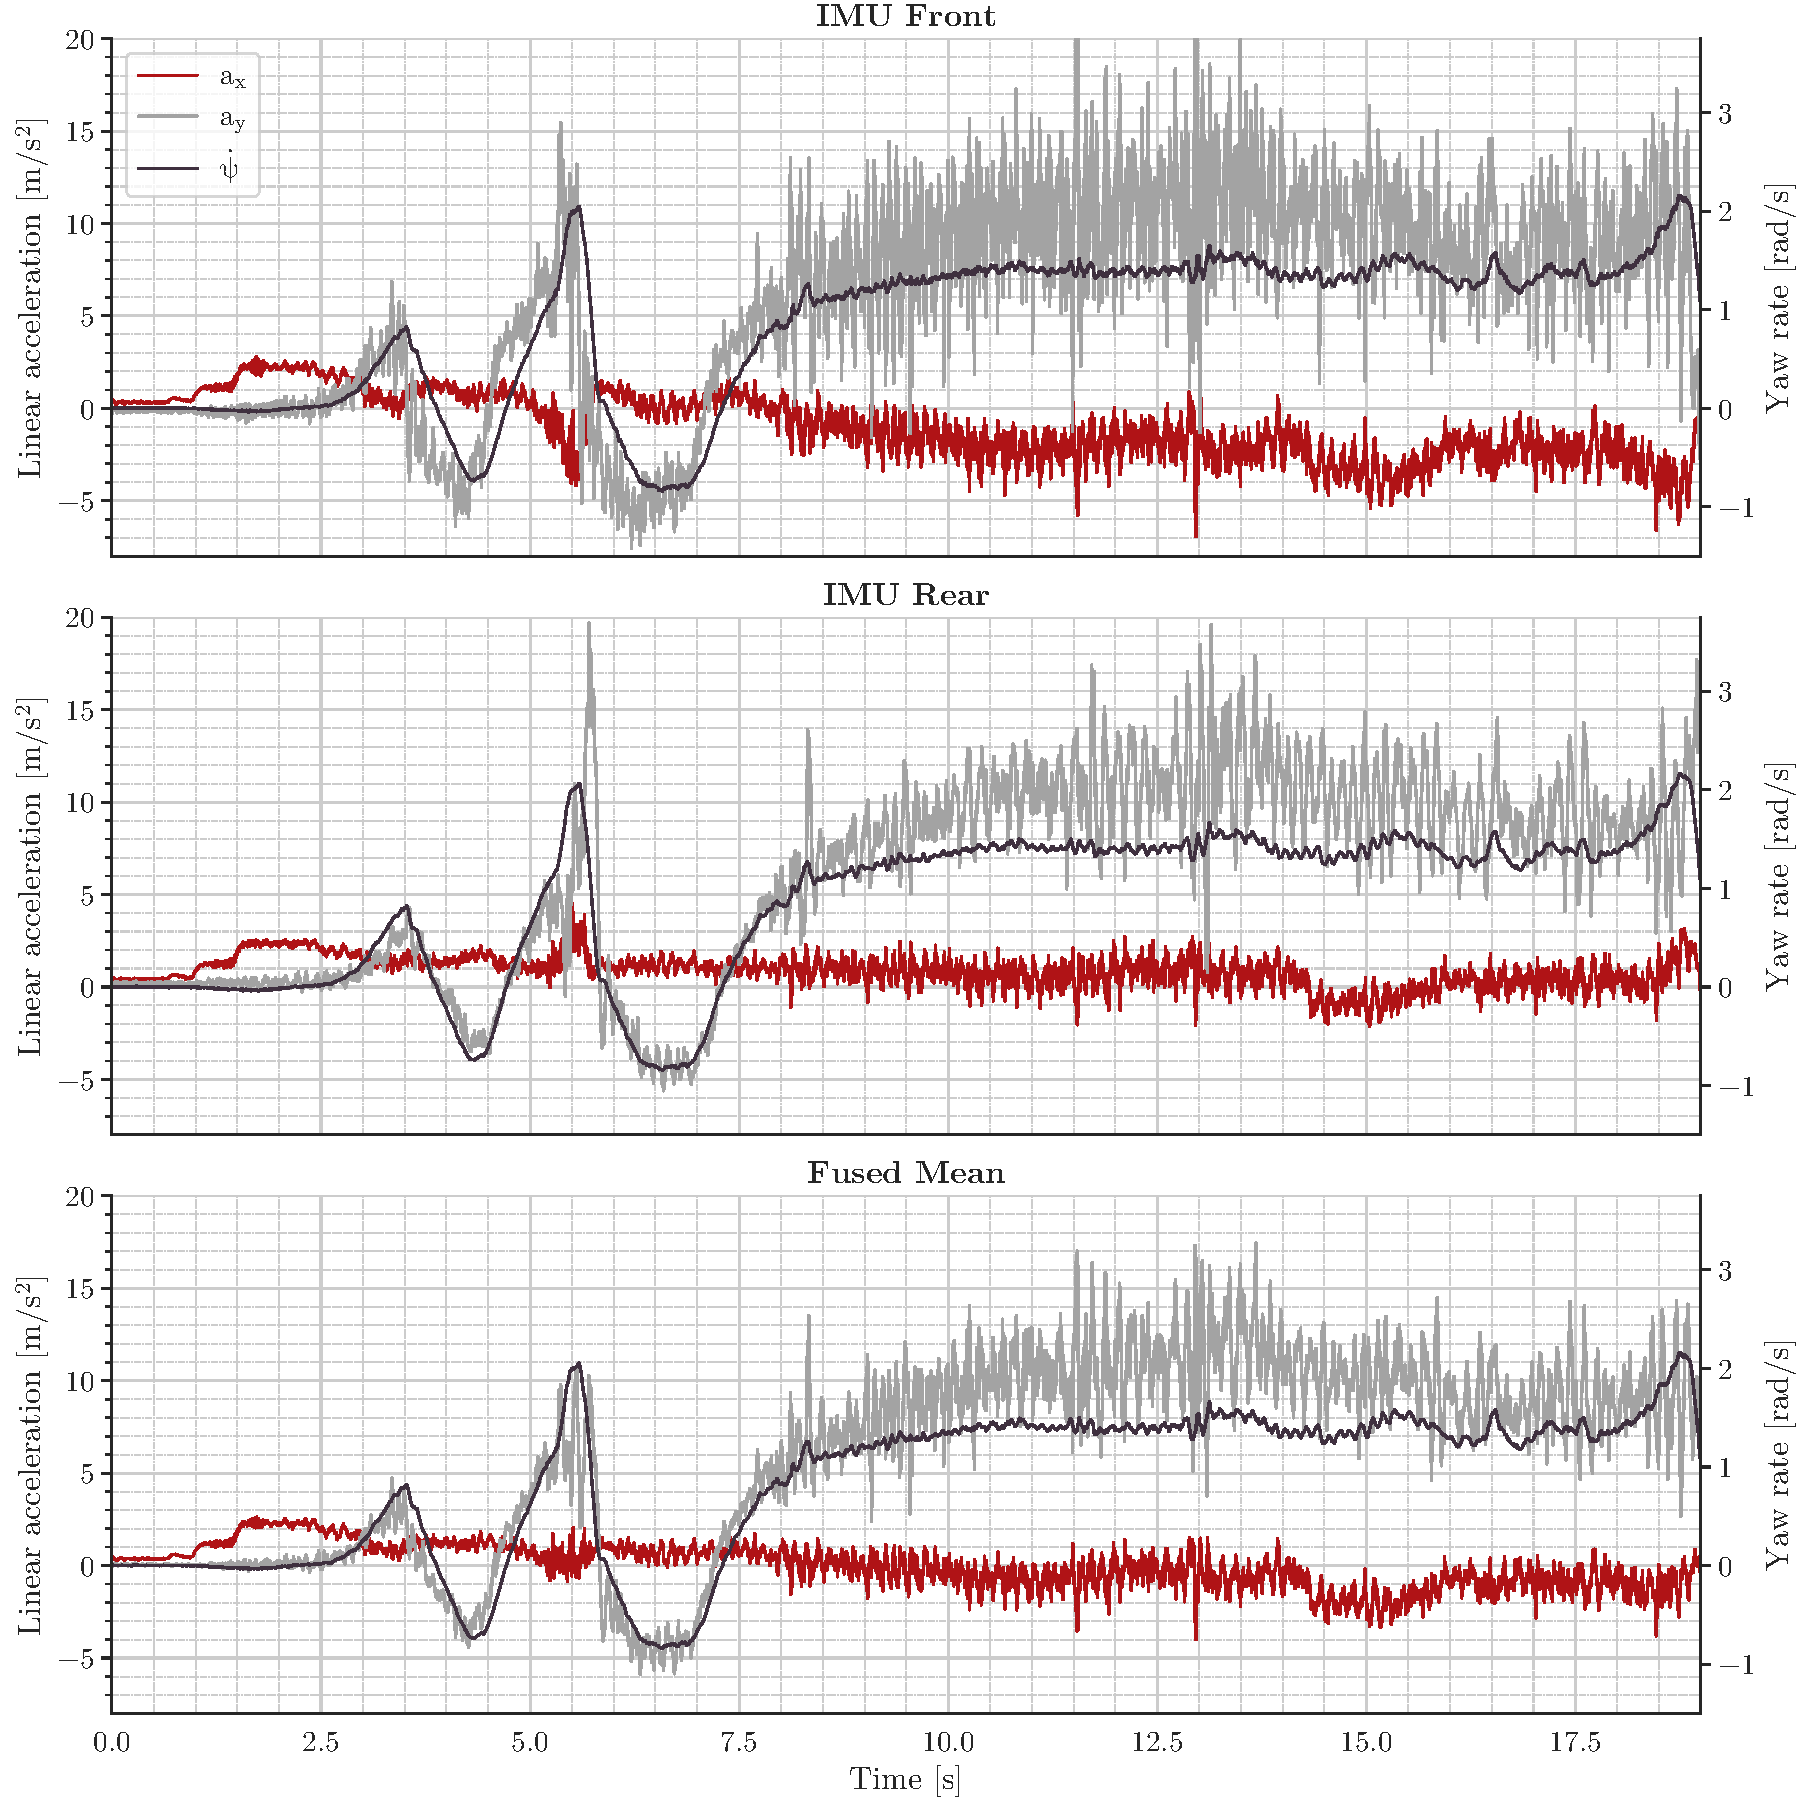
\includegraphics[width=\textwidth]{plot_imu_fusion}%
	\caption{\gls{imu} measurements and fusion results}
	\label{fig:imu-fusion-real}
\end{figure}

\subsection{Failure Detection}

Sanity Check:
compare max change rate and mean based

EKF Bank:
show all wssrs for ekf bank
compare with median outlier detection approaches

\subsection{EKF}

compare raw measurements with velocity estimate
show results for each state variable
effect of different debouncing times and thresholds
show velocity without kistler to simulate dv
bad position in EV without heading measurements, because velocity cannot be used properly to estimate position






\section{Discussion}
Discussion, impact of results on esleek
prepare for DV
initialization of position, maybe not include position when heading is unavailable

imu fusion maybe better with 3 imus and max likelihood
use mean based fusion because occams razor and same results and less computation

only testing can show if outlier detection works, if not maybe try chi-squared test and variance test


